%how to include pdf files in the appendix:
%\cleardoublepage
%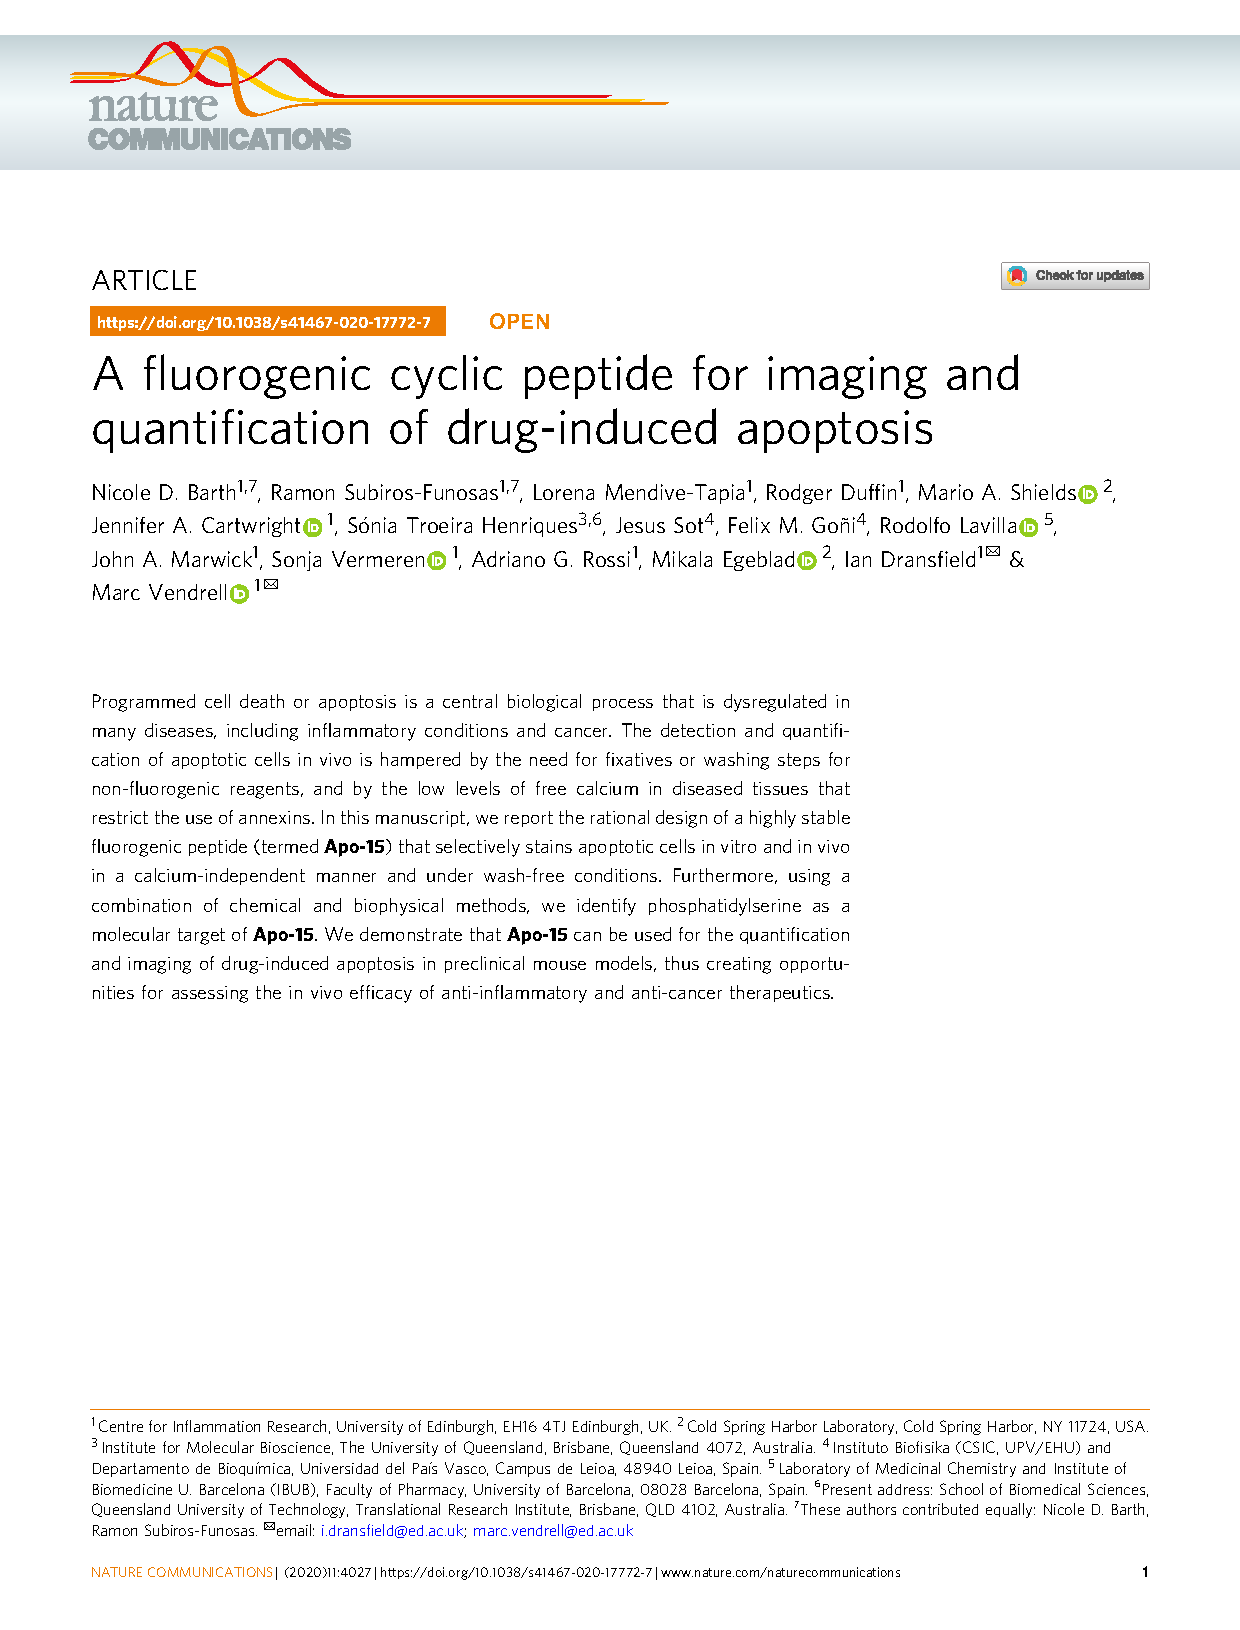
\includepdf[pages=1-2]{appendices/apdfexample.pdf}


%%%%%%%% how to include a note on the bottom of a table in small writing ##########
		%\bottomrule
		%\multicolumn{6}{c}{\footnotesize * Ethanol concentration is above... etc.}
	%\end{tabular}

 ...of aggregation as the sole mechanism causing hemocyte counts to decline with time - 


To test our experimental assumption, two samples from each group were moderately shaken after the last count, such that any free sedimented hemocytes would be resuspended. The samples were rerun directly after. This measure did not increase the number of singlet hemocytes suspended in MAS or ACB, while those in HLS further decreased (data not shown). This suggests that sedimentation is either preceded by irreversible aggregation, or that hemocytes aggregate irreversibly upon sedimentation. 

hich ruled out sedimentation as an important mechani. sm. Hemocytes did sediment with time, but this was Being the only other conceivable mechanism involved, the assumption was regarded as valid under the current experimental conditions.


Aspirate two samples from the same mussel using different buffers to confirm that the hemocyte medium in fact does not change the SSC vs. FSC profiles of the hemocyte subpopulations within 15 minute incubation. Maybe use crude hemolymph as control?
 

Report pH and osmolarity of the MAS and ACB buffer, and say that it is similar to the osmolarity of hemolymph/seawater 990 mOsm (Hartl, 2010).
- The osmolarity of MAS and ACB were adjusted to approximately 990 mOsm by the addition of \ce{NaCl}, to reflect that of \emph{M. edulis} hemolymph (Hartl, 2010)
- This could be co-presented with the fact that cells did not swell during the incubation period, deducted form the fact that the mean FCS-A did not change.

Aggregation can obscure cell type identification and the counting of single haemocytes, such that clumped haemocytes cannot be included in differentials. In addition, clumping seemed to be more severe among basophillic haemocytes, such that an exclusion of clumped haemocytes could potentially skew the differential. To bypass this problem, haemolymph was withdrawn into an equal volume of 5 \% formaldehyde in MPSS, and fixed in suspension for 1 hour. 

 On the basis of the morphological criteria in section \ref{subsection:morph}, the haemocytes where placed in one of three categories: (1) eosinophilic granulocytes, (2) basophilic granulocytes or (3) small blast-like basophils. 


%                            LABORATORY INSTRUMENTS AND SPECS

BD Accuri C6 Plus benchtop flow cytometer (BD Nordics (prev. Puls Norway), Norway). Filters and lasers.
CytoSub submersible flow cytometer (CytoBuoy, Netherlands)
Coulter Counter Multisizer4 (Beckman Coulter, US) eqipped with a 100 \micro m aperture (size-range 2-60 \micro m)

Nikon Eclipse Ni-U
- Semrock Brightline GFP-4050B filter-cube
- Semrock Brightline LED-Cy5-A
- Plan Fluor 40x/0.75 water immersion objective,
- Plan Fluor 100x/1.30 Oil immersion objective

Nikon Eclipse 90i
- Filter specs?
- Nikon Plan Apo 60XA/1.40 Oil immersion objectice
- Nikon Plan Apo VC 100X/1.40 Oil immersion objective

Leitz Labrolux 12 binocular microscope (Leica Mikroskopi AS, Norway) [EF 40/0.65 objective]
Eppendorf Centrifuge 5804 R (Eppendorf, Norway), [rotor: A-4-44, rotor radius: 15.5 cm], high-speed refrigerated benchtop centrifuge
Jouan KR22i floor centrifuge (Thermo Fischer Scientific, US), high-speed high capacity refrigerated floor centrifuge 8 [rotor: AK 100-21] angle?
Bürker Counting Chamber (Hirschmann Laborgeräte, Germany) with 0.1 mm depth of chamber
Eirik Lund sitt kamera, lense og imaging software: 
Sony ILCE A6400 with E-mount, lense: Tamron 17-70mm F/2.8 
Adobe\textsuperscript{\textregistered} Lightroom Classic 12.0 
BD Microlance$^{TM}$ 3, 23G x 1" - Nr. 16, 0.6mm x 25 mm, sterile, REF 300800
HENKE-JECT 1 mL syringes, 1mL, luer, REF 8300014579, HENKE SASS WOLF GmbH, Tuttlingen, Germany

Since no single experiment would convey the amount of variation observed, no experiments were dedicated to characterize the subpopulations quantitatively. A quantitative approach would nor be especially interesting in itself, since the relative units of FSC and SSC vary heavily between instruments and with instrument settings. The exact light-scatter values are only meaningful when measured on the same instrument, and the insights gained from such measurements are mainly pertained to the relative light-scatter profiles of the different subpopulations.

The deviance-based R$^{2}$ is calculated to according to equation to: $R^{2} = 1 \dfrac{Residual ~ deviance}{Null ~ deviance}$. The adjusted deviance-based R$^{2}$ is calculated according to: $Adjusted ~ R^{2} = 1 - \dfrac{n-1}{n-p}(1 - R^{2})$. This was done using the \emph{adjR2()} function of the \emph{glmtoolbox} in RStudio (\cite{RStudio}).

\begin{table}[H]
	\centering
	\caption{Parameter estimates with 95\% CI, Wald z-values and the belonging p-value are presented for the fitted mixed logistic regression model presented in result section \ref{section:Results_Method_Development}.}
	\label{tb:loglogistic_aggregation_oddsratios_copy}
	\resizebox{\linewidth}{!}{
	\begin{tabular}{lccccc}
        \toprule
	\textbf{Covariate} & \textbf{Symbol} & \textbf{Estimate} & \textbf{95\% CI$^{a}$} & \textbf{z-value$^{b}$} & \textbf{Pr(Z > $\mid$ z $\mid)$} \\
		\midrule
  \emph{Intercept}                          & $\alpha_1$ & -1.7192 & [-3.2364, -0.2024] & -2.323 & 0.02    \\
  \emph{log(t)}                             & $\beta_1$  & 0.5516  & [0.1885, 0.9150]   & 3.109  & 0.002   \\
  \emph{Buffer$_{ACB}$}                     & $\alpha_2$ & -5.2650 & [-7.4142, -3.1110] & -5.032 & < 0.0001 \\
  \emph{Buffer$_{MAS}$}                     & $\alpha_3$ & -6.0006 & [-8.1814, -3.8623] & -5.687 & < 0.0001 \\
  \emph{log(t)} $\cdot$ \emph{Buffer$_{ACB}$} & $\beta_2$  & 1.2884  & [0.7749, 1.8000]   & 5.138  & < 0.0001 \\
  \emph{log(t)} $\cdot$ \emph{Buffer$_{MAS}$} & $\beta_3$   & 1.4622  & [0.9492, 1.9841]   & 5.778  & < 0.0001 \\
  \emph{SD}$(\gamma_{0i})$                  & $\tau_0^2$  & 2.0874  & [1.5726, 2.9047]   & -      & -        \\
  \emph{SD}$(\gamma_{1i})$                  & $\tau_1^2$  & 0.5001  & [0.3788, 0.6936]   & -      & -        \\
  &&&&& \\
  \multicolumn{6}{l}{Marginal R$^{2}$ = 0.87} \\
  \multicolumn{6}{l}{Conditional R$^{2}$ = 0.98} \\
  \multicolumn{6}{l}{Residual deviance: 13498 on 98 degrees of freedom} \\
		\bottomrule
  \multicolumn{6}{l}{\footnotesize $^{a}$Profiled 95\% confidence intervals based on the Likelihood Ratio Test.}\\
  \multicolumn{6}{l}{\footnotesize $^{b}$ z-statistics derived from the asymptotic Wald test.}
	\end{tabular}
 }
\end{table}

\begin{figure}[!ht]
    \centering
    \includegraphics[width=1.0\textwidth]{figures/Method development/Eosin fluorescence figure.pdf}
    \caption{\textbf{Eosinophilic granulocytes can be distinguished from the two basophilic cell types according to eosin fluorescence ($\geq$ 515 nm).} Formaldehyde-fixed haemocytes stained in 0.75\% eosin and 3\% Giemsa were imaged at $\times$60 under \textbf{A)} brightfield illumination and \textbf{B)} by epifluorescence microscopy with a B-2A filter cube. The slide was mounted with Eukitt\textsuperscript{\textregistered} and coverslipped prior to microscopy. Eo: eosinophilic granulocyte; B: basophilic haemocyte; scale bars = 10 \micro m. }
    \label{fig:reserve}
\end{figure}

0.14$\pm{0.09}$ and  0.20$\pm{0.12}$


%Buffer  mean   std.dev  df  S.E.     CI_lower   CI_upper
1 ACB    0.142  0.0863   8   0.0305   0.0703    0.215
2 MAS    0.195  0.120    6   0.0488   0.0695    0.321
3 MPSS   0.475  0.0986   8   0.0348   0.393     0.557

MPSS vs. MAS, p = 0.0002139 >
MPSS vs. ACB, p = 0.0000024 >
ACB vs.  MAS, p = 0.3572    diff

During the initial two-hour incubation period, the percentage of necrotic haemocytes in cold MPSS did not change significantly. However, a relatively small increase of 1.18\% was observed during the final 18 hours. C
The percentage of necrotic haemocytes in cold MPSS did not increase during the first two hours of incubation, and showed only a small increase of 1.18\% during the last 18 hours (Table \ref{tb:Paired_ttests}).


Haemolymph was withdrawn from the posterior adductor muscle of 9 adult mussels into an equal volume of methanol (n=3), 3:1 methanol:glacial acetic acid (n=3) or 5\% formaldehyde in \acrshort{mpss} (n=3) and fixed for 30 minutes in suspension. The fixed haemocytes were pelleted by centrifugation (250G, 5 min, \SI{20}{\celsius}) and resuspended in the eosin component of the Hemacolor\textsuperscript{\textregistered} kit. After staining for 5, 10 or 15 minutes, the stained haemocytes were pelleted (180G, 5 min, \SI{20}{\celsius}), resuspended in 100 \micro L Sorensen buffer and transferred onto glass slides. The slides were coverslipped and inspected under brightfield illumination on a Nikon Eclipse Ni-U upright microscope with a 40x/0.75 objective.

In some adult mussels, however, the basophilic and eosinophilic granulocyte subpopulations are partly overlapping with regard to internal complexity, i.e., SSC. Since the BD Accuri C6 Plus isn't equipped with adjustable laser gain settings, these subpopulations could not be separated further instrumentally. Thus, any attempts to gate on these subpopulations based solely on light scattering profiles, would in some mussels introduce considerable uncertainty into their relative proportions. [Find the proportion of mussels where they are not well separated, and report that number instead of saying "some" mussels here.]

When incorporating the Coulter Counter data in this section, this article can be used to reference the accuracy of the electronic cell size method which it uses: Mattern CFT, Brackett FS, Olson BJ. Determination of number and size of particles by electrical gating: blood cells. J Appl Physiol 1957;10:56–70

This is where you write about your results in the context of what was expected, what others with similar experiments have found (in line with, contradictory, similar to). Put it together with other findings that may be relevant or interesting. The results are interpreted: what do they mean for the field, the risk assessors, the environmental risk of Ti2O, ZnO Ag NPs in the aquatic environment, Trondheimsfjorden. Extrapolate to a greater level of organization?. Put the results into a bigger context.


We should have withdrawn two samples from each mussel (as we did), but one into MPSS for staining with the Hemacolor kit and subsequant MN scoring (cold MPSS, 5 min inc in humid chamber) and one into ACB for FCM assays. With a bit dilution in MPSS and short incubation, neither aggregation nor spreading is a problem.

Haemolymph smears can be messy. Therefore, scoring of necrotic and apoptotic haemocytes by microscopy should be performed by certified operators with formal education or practice from hematology or immunology. A few example PNG images with from a published protocol leaves too much to subjectivity. Secondly, if they are rare events (e.g., low dose), why not score all 10 of 100.000 cells objectively by FCM instead of 0 or 1 from 1000 cells in the smear?


\section{The role of hemocytes}
Use articles citing Friebel and Renwrantz (1995) to locate articles that have a characterized these cell-types in therms of enzyme activity and cytochemistry. (E.g. 10.1016/j.jip.2009.10.001).

Functional classification based on phagocytic capacity: Differences in phagocytosis between granulocytes and agranular haemocytes may be related to the type of phagocytosed particles involved, rather than differences in phagocytic ability (Hine, 1999)

Unlike granulocytes and hyalinocytes, precursor cells do not contribute to immune-response mechanisms such as phagocytosis or encapsulation, and they also lack common intracellular enzyme systems associated with host defence. 

Their lack of cytoplasmic organelles seems to preclude a secretory or phagocytic function

Basophilic cytoplasm suggest the presence of free ribosomes and immaturity

Refer to the 1990 study of Pipe when explaining the functions of the cytoplasmic granules.

Hemocytes also (in addition to lung and digestive gland) showed high expression levels (of initiator and executioner caspases), probably due to the role of apoptosis in the defense against pathogens. Because bivalves are highly susceptible to climate changes, pollutants and pathogens, it  could be suggested that a strong apoptotic process may be necessary to ensure body homeostasis. (Romero, 2011). See page 11 of (New Insights into the Apoptotic Process in Mollusks: Characterization of Caspase Genes in Mytilus galloprovincialis) for greater detail and references.



\section{Method}
\subsection{Animal housing}
Here, the mussels were kept to acclimatize for 2 days before transfer to the experimental exposure setup.
"were fed twice a day with a mixed diet (Chaetoceros sp. and Thalassiosira sp.). Mussels were maintained in locally-sourced seawater, which was sand-filtered and allowed to settle in the dark prior to use. Sand-filter, protein-skimmed and UV-treated."

Time of mussel harvest/purchase?

Describe water treatment in more detail: include information regarding sand-filter, protein-skimmer, 0.5 um filter bags and UV-treatment.

Because the watertreatment left no natural feed for the mussels, the filtered seawater were supplemented with algae [insert species \& frequency].


\subsection{Experimental setup/design}
- Specs related to flowrate, feeding (alge conc: Coulter counter), how often was nano particles changed (every 3-4 days: check article), concentrations (ICP-MS --> mg/L in stocks and exp tanks), zetasizer --> size and surface potential

include figure of exp setup?

depuration period: check article

storage from depuration to sampling: mussels were not kept on ice, but were washed and taken directly upstairs for measuring weight, length, height and width for condition index, and were given to us for \acrshort{fcm} sampling afterwards. If we were delayed, they were kept in the fridge until hemolymph sampling 

\subsection{Hybrid Micronucleus Assay}
Sampling
Flow Cytometer used and Flow Cytometry acquisition software
External software used for graphing and analysis of exported FCS files.
Replicate/triplicate measurements?
Number of events recorded for each mussel?
Briefly describe FCS and \acrshort{ssc}.
Mention if data were collected in linear or logarithmic scale, 
FSC treshold (80.000 FSC-H). 
Fluorescent compensation (matrix)
Describe gating strategy herein? Debris exclusion (size); doublet exclusion --> haemocytes. (Gating of basophils and eosinophils, the use of \acrshort{fmo} controls with TO-PRO-3 and/or the apoptosis stain) to create gates.

\subsubsection{Scoring of necrotic haemocytes}

\subsubsection{Scoring of apoptotic haemocytes}

\subsubsection{Differential haemocyte count}

\subsubsection{Determination of haemocyte concentration}

\subsubsection{Slide preparation}
Refer to the MN cytome assay by Bolognesi, and mention that we fixed and stained haemocytes in suspension to produce slides without aggregated haemocytes. Since the cells were dead, they did not spread or produce pseudopodia, which allowed us to observe the actual size and form which they would posses ass they flowed through the laser of the flow cytometer.

\subsubsection{Scoring of MN and nuclear anomalies}

\subsubsection{Reference toxicity}
Baseline group.

\subsubsection{Measurements and calculations}
(\cite{R-project})

\subsubsection{Statistical analysis}


The complete list of endpoints required scoring data are presented in table (Insert table ref)

Low toxicity: Calcein/AM induced no immediate loss (3 h) of membrane integrity (10.1097/00001813-199508000-00011).


The correlation between the flow cytometric estimates and microscopic counts were tested by simple linear regression. In order to evaluate the accuracy of the gating strategy, the \acrshort{mae} of the estimates were calculated relative to the microscopic counts.

The results are presented and discussed consecutively since each subsequent section builds on the preceding.

Since Le Foll and colleagues (2010) reported that the motile properties of the different haemocyte subpopulations of \emph{M. edulis} could be used as an additional functional criteria for their characterization, the spreading behavior of the different cell types were included to expand on the morphological characteristics. This comprehended a description of the typical haemocyte shapes and motile structures that were observable under differential interference contrast illumination in spread haemocytes. The preparation of slides with spread haemocytes followed a methodology similar to that of the non-spread haemocytes, but the humid chamber incubation periods prior to fixation and staining were extended (15-30 min). Microscopic fields were examined through a 60$\times$/1.40 oil immersion objective under DIC illumination.

\begin{table}[h!]
\centering
	\caption{Bla bla}
	\label{tb:linmod}
        \resizebox{\linewidth}{!}{
	\begin{tabular}{lcccc}
		\toprule
		\multirow{2}{*}{Microscopy} & \multicolumn{2}{c}{\textbf{Flow cytometry}} & \multirow{2}{*}{MAE (\%)} & \multirow{2}{*}{R^$^{2}$}\\
		& FSC vs. log SSC & log calcein vs. log SSC & & &\\
		\midrule
     Small blast-like basophils & Cluster 1 & Calcein$^{-}$/SSC low  & 0.70 & 0.92 \\
     Basophilic granulocytes    & Cluster 2 & Calcein$^{-}$/SSC mid  & 2.83 & 0.96 \\
     Eosinophilic granulocytes  & Cluster 3 & Calcein$^{+}$/SSC high & 2.93 & 0.97 \\
		\bottomrule
	\end{tabular}
 }
\end{table}


[This part is potentially removed if the above bridge is chosen] Their feeding strategy in particular make them highly effective in micro- and nano-scaled particle uptake (\cite{Canesi2012}), which has led to their use in a large pool of studies on the effects of engineered nanoparticles (\cite{Rocha2015}). These studies often integrate a battery of cellular and molecular biomarkers of pollutant-induced stress and immunomodulation, where the \acrshort{mumncyt} assay is included to evaluate potential cytogenotoxic effects (see e.g., \cite{Rocha2014, Ruiz2015}).

It is a suspension feeder, filtering high quantities of water for suspended particulate matter (\cite{Beyer2017b}). This feeding strategy makes them highly effective in micro- and nano-scaled particle uptake, and consequently especially susceptible to engineered NP exposure (\cite{Canesi2012}). \emph{Mytilus sp.} 53.4\% of papers related to ecotoxicity of ENMs until december 2014 (\cite{Rocha2015}).

this marine invertebrate represents a suitable system for monitoring and assessing the impacts of anthropogenic pollution on the health of marine coastal ecosystems. Furthermore, they... [Concider bridging with their key ecological, commercial importance and suceptibility to bachteria - which has caused population declines in France, Spain with examples: 

Unlike oysters and clams, which also represent bivalve molluscs of major ecological and economical interest, mussels are actually not subjected to episodes of massive mortality (\cite{Costa2009} in: \cite{Rioult2014}).

Important commercial species and a KEY component of marine coastal ecosystems: \emph{Mytilus spp.}: blue mussels are ecologically important as they provide essential ecological services such as food and habitat to a multitude of other species. In: Beyer et al., 2017.


\subsubsection{Differential count: granular and agranular haemocytes per 1,000} %cytometric marameters = THC and DCC
In addition to scoring cytogenic damage (MNi and NBUDs) and cytotoxic alterations (necrosis/apoptosis), the protocol includes a differential count of agranular and granular haemocytes (per 1,000).

Just a theory: Given that the blast-like cells are the precursor of both granular cell types, and chemical insult leads to increased proliferation of blast-like cells - which increases the risk of neoplastic cells (prolif rate pos. corr. to mutations). Increased recruitment/hamatopoiesis/cell turnover rate

Since their basophilia indicates the presence of free ribosomes and immaturity, while their lack of cytoplasmic organelles precludes a secretory or phagocytic function, these cells are thought to represent the immature "prohemocyte" precursor of one or both granular cell types (\cite{Hine1999})

- Seasonal variation in agranular and granular (\%) haemocytes in M. galloprovincialis (\cite{Santarem1994}). May be related to reproduction/spawning (allocation of resouses/nutrients?)

genotoxic disease syndrome (\cite{Kurelec1993}) through increased mutational rates


READ LIVINGSTONE et al, 2000: immune response


Cd:
- Decrease in eosinophilic granulocytes in response to Cd QDs, while basophils increased in response to Cd2+. (Basopils incl. blasts). Suggested limitation of QD transport by EO, since they decreases (\cite{Rocha2014}). May offer insights into the target/susceptible cell-types in NP toxicology, which may indicate possible immunomodulating effects. % M. edulis
- Increased numbers of small hyaline (blast-like) cells within the hyalinocyte sub-population of C. gigas, following exposure to 0.3 ppm cadmium ions, with a concomitant decrease in large cells (\cite{Auffret1994}). THC increased with time of exposure relative to control (2x increase). % C. gigas
- THC increased following exposure to Vibrio tubiashi after preexposure with Cd (\cite{Pipe1995}) % M. edulis



Cu2+  
- Cu2+ + Vibrio tubiashi led to sig. decrease in eosinophils compared to basophils. No such effect was observed with Cd or fluoranthene (\cite{Pipe1995}) % M. edulis
- 0.2 and 0.5 ppm Cu2+ decreased the proportion of eosinophilic to basophilic cells (\cite{Pipe1999})

  PAHs
- Basophilic haemocytes freq. showed sig. negative correlation with PAH concentrations after oil spill, while EO showed a sig. positive correlation. Inverse corr. between 3 PAHs and THC. Immune parameters decreased, while EO increased: possible compensatory effect? No time-related effects (\cite{Dyrynda1997}). Small hyaline cells were positively correlated with total PAHs conc. mm. (never neg corr.) % M. edulis
- Dyrynda (1998) THC and DCC (Eo \%). No sig. diff beteen contaminated site and ctrl, but slight deacrease in both. Argues that immunomodelation did not arise from THC or DCC changes. Observed in laboratory settings with sudden short-term exposure, but may adjust to longterm exposures.  (\cite{Dyrynda1998}) Did not score blast-like cells % M. edulis 

\subsection{The role of haemocytes}
Present the difference in phagocytic capacity between the three cell types (include different types of materials).
Cytochemistry, enzyme content and cytotoxic secreted molecules in host defence, Surface receptors.
Ultrastructural findings: what organelles are found in the different cell types, and what they suggest about function.
The  eosinophilic granular cells in  M. edulis are the most active in phagocytosis and superoxide production (Pipe  et al., 1997)

Mussel hemocytes represent a valuable model of invertebrate innate immune cells, in which potential immunomodulating effects of xenobiotics can be assessed. Formulation from \cite{Rioult2014}.

Next paragraph: The MUMNcyt assay represents a well "bla bla" assay, capable of uncovering potential immunomodulating effects of toxicants, as well as the underlying mechanisms of these shifts (apoptosis/necrosis). 

- Renwartz L. Variations in hemocyte counts in the mussel, Mytilus edulis: Similar reaction patterns occur in disappearance and return of molluscan hemocytes and vertebrate leukocytes. (2013)

Theory behind Annexin-V/Apo-15 Annexin V has affinity for phosphatidylserine, which is externalized to the outer layer of the plasma membrane in the earlier stages of apoptosis to facilitate recognition by macrophages (\cite{Fadok1992}). ATP/Mg2+ dependent process (\cite{Connor1992}). Annexin V also binds internal phosphatidylserine (\acrshort{ps}) in permeable membranes, i.e. dead cells. Thus, dead cells are Apo-15+ ToPro3+, while the early apoptotic cells are only Apo15+. The Annexin V/PI assay is considered the the gold standard of \emph{in vitro} monitoring of cell death (\cite{Jiang2016}), but requires free Ca$^{2+}$.

ATP/Mg2+ dependent process (\cite{Connor1992}). Since EDTA chelates Mg2+ and Ca2+, there will be less development of the PS translocation to the outer membrane leaflet during staining, but will rather reflect the proportion of apoptotic cells from the sampling point.

This section describes in detail the work and experiments that were performed in the development of a hybrid flow cytometry- and microscopy-based version of The Mussel Micronucleus Cytome Assay by Bolognesi and Fenech (2012). The finalized assay is presented in it's entirety in the method section, in the context of it's application to test the potential genotoxic and cytotoxic effects of aged \ce{TiO2} and Ag \acrshort{ENPs}. The results from this section is presented in a separate results chapter (5), which can be beneficial to read through before continuing with the method section and the main results (6).

Include some technical stuff? E.g., unless stated otherwise, 10.000 events were acquired from each sample with 36 uL/min and 16 \micro L core size. 80.000 FSH-H was used as the only threshold, and doublet haemocytes were gated out of analysis with a FSH-H vs FSC-A singlets gate.

The images were captured using a Sony A6400 mirrorless digital camera with a Tamron 17-70mm F/2.8 lens, and were edited with Adobe\textsuperscript{\textregistered} Lightroom Classic 12.0 image editing software.

of elimination of amplified DNA and/or DNA repair complexes

Bjørns forlsag: "Since a flow cytometric approach has great potential to improve the power and efficiency of the existing methodology - while creating less room for subjectivity - the aim of the present MSc thesis was to develop a hybrid flow cytometry/microscopy protocol of the micronucleus cytome assay by Bolognesi and Fenech."

Along with the formation of DNA-adducts and strand-breaks, the induction of micronuclei (\acrshort{mni}) represent one of few availible biomarkers of genotoxicity that are considered relevant to the Ecosystem Approach principle employed in monitoring and assessment of biological effects data by the

A broader and more general introduction, focusing on contamination and genotoxic chemicals, followed by the need to monitor hazardous effects of contaminants in the marine environment (aim/purpose of testing, hva er det vi prøver å oppnå/unngå?), and that the MN assay is a used a lot for this purpose. Bridge with the need of sensitive and reliable (standardized) assays to monitor the health of our coastal environments, and to assess the effectiveness of coastal remediation projects (maybe cite article 17-18 in Bolognesi). Regulate the production, use and emission of ... locally, nationally or internationally. Spatial and temporal trends. Trekk in FN sustainebility goals?


\begin{table}[H]
	\centering
	%\caption{Reagents and kits used in the master thesis, listed alphabetically according to product name, including manufacturer, supplier and supplier's catalogue number.}
	\label{tb:Microscope_software-list}
	\resizebox{\linewidth}{!}{
	\begin{tabular}{lll}
	\textbf{Equipment} & \textbf{Model} & \textbf{Manufacturer} \\
		\midrule
   \multicolumn{3}{l}{\textbf{Setup for Nikon 90i:}} \\
   Microscope controller software           & iControl v.2.0.0.3        & Nikon Corp \\          
   Light engine                             & EL6000                    & Leica Microsystems \\
   Microscope camera                        & DS-Fi1                    & Nikon Corp\\
   DS-Fi1 camera controller                 & DS-U2                     & Nikon Corp \\
   DS-Fi1 digital imaging software          & NIS Elements D v.3.22.15  & Nikon Corp \\
   Microscope camera                        & DS-Fi1c                   & Nikon Corp \\
   DS-Fi1c camera controller                & DS-U3                     & Nikon Corp \\
   DS-Fi1c digital imaging software         & NIS-Elements F v.4.60     & Nikon Corp \\
   Flat top microscope stage                & Proscan H101/2            & Prior Scientific \\
   Microscope stage encoder                 & Lie5 1P N2KV              & Numerik Jena \\
   Microscope stage controller              & Proscan II                & Prior Scientific\\
   Filtercube                               & Brightline\textsuperscript{\textregistered} Led-Cy5-A  & Semrock \\
   Filtercube                               & B-2A                      & Nikon Corp \\
   Stage micrometer cal. slide              & 2 mm, 0.01 mm interval    & Leitz \\
   Objective lens                           & Plan Apo 20X/0.75         & Nikon Corp \\
   Objective lens                           & Plan Apo 60XA/1.40 Oil    & Nikon Corp \\
   Objective lens                           & Plan Apo VC 100X/1.40 Oil & Nikon Corp\\
   
   && \\
   \multicolumn{3}{l}{\textbf{Setup for Nikon Ni-U:}} \\
   Light engine                             & Sola SM II 365            & Lumencor Ink. \\
   CMOS camera                              & MC170HD                   & Leica Microsystems \\
   Microscope camera                        & 4KHDMI                    & DeltaPix \\
   Objective lens (Nikon Ni-U)              & Plan Fluor 40X/0.75       & Nikon Corp \\
   Objective lens (Nikon Ni-U)              & Plan Fluor 100X/1.30      & Nikon Corp \\
		\bottomrule
	\end{tabular}
	}
\end{table}